%%%%%%%%%%%%%%%%%%%%%%%%%%%%%%%%%%%%%%%%%%
%% TEX main file for the CLAS12 Nim Papers
%%       Do not edit this file
%%%%%%%%%%%%%%%%%%%%%%%%%%%%%%%%%%%%%%%%%%
%\documentclass[3p,times]{elsarticle}
\documentclass[3p,times,twocolumn]{elsarticle}
\usepackage{lineno, hyperref, color, xspace, pdfwidgets, enumerate, amssymb, graphicx, float, wrapfig, listings}
\usepackage[section]{placeins}
\modulolinenumbers[5]
\linenumbers

\lstset{
basicstyle=\ttfamily\small
}

\journal{Nuclear Instruments and Methods A}

\newcommand{\F}[1]{Fig.~\ref{fig:#1}}

\begin{document}

\begin{frontmatter}
\title{Micromegas Vertex Tracker for CLAS12}

\author[A]{A. Acker} 
\author[A]{D. Atti\'e}
\author[A]{S. Aune}
\author[A]{J. Ball}
\author[A]{P. Baron}
\author[A]{Q. Bertrand}
\author[A]{D. Besin}
\author[A]{T. Bey}
\author[A]{F. Boss\`u}
\author[A]{R. Boudouin}
\author[A]{M. Boyer}
\author[A]{G. Charles}
\author[A]{G. Christiaens}
\author[A]{P. Contrepois}
\author[A]{M. Defurne}
\author[A]{E. Delagnes}
\author[A]{M. Garçon}
\author[A]{F. Georges}
\author[A]{R. Granelli}
\author[A]{N. Grouas}
\author[A]{C. Lahonde}
\author[A]{T. Lerch}
\author[A]{I. Mandjavidze}
\author[A]{O. Meunier}
\author[A]{Y. Mouden}
\author[A]{S. Procureur}
\author[A]{M. Riallot}
\author[A]{F. Sabati\'e}
\author[A]{E. Virique}
\author[A]{M. Vandenbroucke}



\address[A]{Irfu, CEA, Universit\'{e} Paris-Saclay, 91191, Gif-sur-Yvette, France}

\begin{abstract}

For the 12 GeV upgrade of Jefferson Laboratory, a Silicon Vertex Tracker (SVT) has been designed for the CLAS12 spectrometer using single-sided microstrip sensors fabricated by Hamamatsu. The sensors have a graded angle design to minimize dead areas and a readout pitch of 156 $\mu$m, with intermediate strips. Each double-sided SVT module hosts three daisy-chained sensors on each side with a full strip length of 33~cm. There are 512 channels per module, read out by four Fermilab Silicon Strip Readout (FSSR2) chips, featuring data-driven architecture, mounted on a rigid-flex hybrid board. The modules are assembled on the barrel using a unique cantilevered geometry to minimize the amount of material in the tracking volume. This paper is focused on the design, qualification of the performance, and experience in operating and commissioning the tracker during the first year of the data taking.

\end{abstract}

\end{frontmatter}

\date{\today}

% added to verify: ec and ltcc

\section{Overview}

simulations overview description, how geometry and digitization.

Then we go to each detector

- geometry
- calibration constants
- digitization.





\subsection{Target}

The CLAS12 target components are imported from the engineering model. The STEP files are converted to tessellated STL files and imported
in the GEMC simulation \cite{targetCorrection}, \cite{targetStudy}. An example of the tessellation is shown in \F{targetScatteringChamber}.

Key elements of the STL import include the torlon tube to the target cell,
the target aluminum windows, the Kapton walls, and the scattering chamber, see \F{targetDesign}.
An overview of the target in Geant4 and the engineering model is shown in \F{targetOverview}.

\begin{figure}
	\centering
	\includegraphics[width=0.95\columnwidth,keepaspectratio]{img/targetDesign.png}
	\caption{The CLAS12 target design. Top left: the entry assembly schematic. Top right: the liquid hydrogen cell
            dimensions: the outer radius is tapered down from 15 mm at z=-2.5cm to 10mm at z=2.5mm.
            Bottom left: The cell implementation in GEMC from the CAD drawings. From left to right (beam direction):
            the black torlon tube, the upstream aluminum window, the target cell, the kapton cup and the
				downstream aluminum window. Bottom right: the GEMC implementation of the kapton cup.}
	\label{fig:targetDesign}
\end{figure}


\begin{figure}
	\centering
	\includegraphics[width=0.99\columnwidth,keepaspectratio]{img/targetOverview1.png}
	\includegraphics[width=0.99\columnwidth,keepaspectratio]{img/targetOverview2.png}
	\caption{Top: overview of the target implementation in GEMC includes the scattering chamber (cyan color), the
            downstream cup near the right of the figure and 50 $\mu$m aluminum window. Bottom: the torlon base
            tube starts at a radius of r=6.06 mm, and ends at r = 7.75 mm. It is 63.7 mm long.}
	\label{fig:targetOverview}
\end{figure}

The Github location of the GEMC perl API scripts and the STL files is \url{https://github.com/gemc/detectors/tree/master/clas12/targets}.






\section{Barrel Silicon Vertex Tracker (BST)}

The CLAS12 BST geometry is created using the geometry service (location?)
The geometry directory is "bst".


\subsection{Geometry}

\subsubsection{Geometry Git Location}

\subsection{Process ID}

\subsection{Digitization}


\subsubsection{ADC}
\subsubsection{TDC}

\subsubsection{Summary of CCDB Table used}

\subsection{Digitized Bank}

\subsubsection{Time Window}

\subsubsection{Process Routine Git Repository Location}


The BST hit process routines are located in the repository: \url{https://github.com/gemc/source/tree/master/hitprocess/clas12/svt}

\subsection{Barrel and Forward Micromegas Trackers (BMT and FMT)}

\subsubsection{Geometry}

The Micromegas geometry is implemented through the native GEMC geometry API. There are two subsystems: a ``barrel'' micromegas
between the SVT and the CTOF, made by are three concentric regions divided azimuthally in three identical sectors; and a ``forward'' micromegas
made by three disk regions divided azimuthally in six identical sectors. In both subsystems each region is made by two layers,
one with wires parallel to the beam and one with wires perpendicular to the beam (see \F{bmtGeometry}).
Each micromegas sector contains a cover layer with copper ground, the printed circuit board (PCB) with the readout strips,
the Kapton support, the mesh layer, the ionizing gas, and other layers of material, listed in order below:

\begin{itemize}
	\item overlay
	\item copper ground
	\item PCB
	\item strips
	\item Kapton
	\item gas (amplification gap)
	\item mesh
	\item gas (drift detection gap)
	\item drift potential electrode
	\item foil
	\item ground
\end{itemize}

The sensitive volume contains argon/isobutane gas and is associated with the BMT and FMT hit process routines.
The geometry is summarized in \F{bmtGeometry}. The strip identification is performed in the Process ID routine.

\begin{figure}
	\centering
	\includegraphics[width=0.99\columnwidth,keepaspectratio]{img/bmtGeometry.png}
	\includegraphics[width=0.99\columnwidth,keepaspectratio]{img/bmtDetail.png}
	\caption{Top: a longitudinal cut view of the CLAS12 Central Detector trackers. The target is surrounded by 3 layers of SVT and
            6 layers of micromegas, 3 with $z$-strips, 3 with $c$-strips. On the downstream end (beam incident from the left)
			the Forward Micromegas Tracker disks are visible.
            Bottom: detail of the micromegas GEMC geometry, showing the overlay cover, the copper ground, and the PCB.}
	\label{fig:bmtGeometry}
\end{figure}


\subsubsection{Process ID}
At each Geant4 step, the local coordinates in the sensor volume are used to calculate the strip number.
The algorithm includes the Lorentz angle based on the magnetic field strength, the particle direction,
the pitch angle between the strips, and the dead zones of the sensitive parts.
A virtual electron avalanche is simulated based on the energy deposited. The avalanche
is deposited onto one strip or distributed among several to account for the energy sharing.



\subsubsection{Digitization}

The Micromegas digitization provides the ADC value calculated using the total energy deposited (after hit sharing).
There is no timing information in the output.
The digitized output bank variables are summarized in Table \ref{tab:mmBank}.

\begin{table}[h]
	\begin{center}
		\begin{tabular}{| c | c | c |}
			\hline \hline
			Variable & Description  \\
			\hline
              layer  &      layer number   \\
             sector  &     sector number   \\
              strip  &      strip number   \\
               Edep  &  energy deposited   \\
                ADC  &               ADC   \\
			\hline \hline
		\end{tabular}
	\end{center}
	\caption{The digitized BMT and FMT banks.}\label{tab:mmBank}
\end{table}

The time window  of the Micromegas is set to to 132 ns: all Geant4 steps within the same strip and time window are collected in one hit.


\section{Central Time-Of-Flight (CTOF)}

The CLAS12 CTOF geometry components are imported from the engineering model. The cad files are converted to tessellated STL files.
The geometry directory is "ctof"

\subsection{Geometry}

\subsubsection{Geometry Git Location}

\subsection{Process ID}

\subsection{Digitization}

\subsubsection{Summary of CCDB Table used}

\subsection{Digitized Bank}

\subsubsection{Time Window}

\subsubsection{Process Routine Git Repository Location}



\subsection{Central Neutron Detector}

The Central Neutron Detector (CND)~\cite{cnd-nim} reconstruction service is designed to process raw ADC and TDC information and reconstruct clusters, defined as ensembles of counters matched in space and time. These objects constitute the output of the service that is passed to the Event Builder for particle formation and identification. The algorithm implemented in the service include three steps:

\begin{itemize}
\item{the reconstruction of the time and position of the hit in the paddle;}
\item{the reconstruction of the deposited energy;}
\item{the matching of CND hits with tracks coming from the interaction vertex.}
\end{itemize}

%The reconstruction makes use of the calibration constants of the CND summarized in
%Table~\ref{table_cnd_constants}.
%
%%%%%%%%%%%%%%%%%%%%%%%%%%%%%%%%%%%%%%%%%%%%%%%%%%%%%%%%%%%%
%\begin{table}[htbp]
%\begin{center}
%\begin{tabular}{|c|c|c|} \hline
%Constant Name & Number of Constants  & Units \\ \hline
%$t_{\rm{LR}}$ & 72 & ns\\ \hline
%v_{\rm{eff}}$ & 144 & cm/ns \\ \hline
%$u_{\rm{t}}$ & 72 & ns \\ \hline
%$t_{\rm{LR}_{\rm{ad}}}$ & 72 & ns \\ \hline
%$t_{\rm{off}}$ &72 & ns\\ \hline
%$A_{\rm{L}}$ & 144 & cm\\ \hline
%$MIP_{\rm{D}}$, $MIP_{\rm{I}}$ & 144 each & no units \\ \hline
%\end{tabular}
%\caption{The constants computed in the CND calibration.}
%\label{table_cnd_constants}
%\end{center}
%\end{table}
%%%%%%%%%%%%%%%%%%%%%%%%%%%%%%%%%%%%%%%%%%%%%%%%%%%%%%%%%%%%

%\subsubsection{Timing Calibration}
%
%The paddle in which the hit occurs must be determined before all other reconstruction steps. The raw hit
%times are obtained from the measured TDC channel using a slope constant of 0.0234~ns/channel for all
%channels.
%
%The left and right times of a hit in the left paddle (we label them as $t_{{\rm{L}}/{\rm{L}}}$ and
%$t_{\rm{R}/{\rm{L}}}$ where the first index corresponds to the paddle under exam, while the second indicates
%the paddle in which the primary hit happened) are given by:%
%
%\begin{equation}
%\label{eq_time_hit_lr}
%t_{{\rm{L}}/{\rm{L}}}=t_{\rm{off}}+t_{\rm{tof}}+\frac{z}{v_{\rm{eff}_L}}+t_{\rm{S}}+t_{\rm{off}_{\rm{L}}}+{\rm{TDC}}_{\rm{j}},
%\end{equation}
%
%\begin{equation}
%\label{eq_time_hit_lr1}
%t_{{\rm{R}/{\rm{L}}}}=t_{\rm{off}}+t_{\rm{tof}}-\frac{z}{v_{\rm{eff}_L}}+\frac{L}{v_{\rm{eff}_L}}
%+\frac{L}{v_{\rm{eff}_{\rm{R}}}}+u_{\rm{t}}+t_{\rm{S}}+t_{\rm{off}_{\rm{R}}}+{\rm{TDC}}_{\rm{j}},
%\end{equation}
%
%\noindent
%where $t_{\rm{tof}}$ is the time of flight, $z$ is the position of the hit measured from the upstream end of the
%paddle, $L$ is the length of the paddle, $t_{\rm{S}}$ is the start time of the event, $t_{\rm{off}_{\rm{L}}}$ and
%$t_{\rm{off}_{\rm{R}}}$ are time offsets associated to the left and right coupled paddles, and ${\rm{TDC}}_{\rm{j}}$
%is the TDC clock jitter. Similarly if the hit happened in the right paddle one can write:
%
%\begin{equation}
%  t_{{\rm{L}}/{\rm{R}}}=t_{\rm{off}}+t_{\rm{tof}}-\frac{z}{v_{\rm{eff}_{\rm{R}}}}+\frac{L}{v_{\rm{eff}_L}}
%  +\frac{L}{v_{\rm{eff}_{\rm{R}}}}+u_{\rm{t}}+t_{\rm{S}}+t_{\rm{off}_{\rm{L}}}+{\rm{TDC}}_{\rm{j}},
%\end{equation}
%
%\begin{equation}
%t_{R/R}=t_{\rm{off}}+t_{\rm{tof}}+\frac{z}{v_{\rm{eff}_{\rm{R}}}}+t_{\rm{S}}+t_{\rm{off}_{\rm{R}}}+{\rm{TDC}}_{\rm{j}}.
%\end{equation}
%
%Defining $\Delta$ and $\Delta'$ as:
%
%\begin{equation}
%\Delta=\frac{L}{v_{\rm{eff}_L}}-\frac{L}{v_{\rm{eff}_{\rm{R}}}},
%\end{equation}
%
%\begin{equation}
%\Delta'=t_{\rm{L}/{\rm{X}}}-t_{\rm{R}/{\rm{X}}}+t_{\rm{off}_{\rm{R}}}-t_{\rm{off}_{\rm{L}}},
%\end{equation}
%
%\noindent
%where the index X can be R or L, one can compute $\Delta-\Delta'$ for both cases (hit in the left paddle or hit
%in the right paddle). If the hit is in the left paddle:
%
%\begin{equation}
%\Delta'-\Delta= \frac{2z}{v_{\rm{eff}_L}} - \frac{2L}{v_{\rm{eff}_L}} -u_{\rm{t}} <0.
%\end{equation}

%\noindent
%If the hit is in the right paddle:
%
%\begin{equation}
%\Delta'-\Delta= \frac{2L}{v_{\rm{eff}_{\rm{R}}}}-\frac{2z}{v_{\rm{eff}_{\rm{R}}}} +u_{\rm{t}} >0.
%\end{equation}
%
%\noindent
%If $\Delta'<\Delta$, the paddle in which the hit happened is the left one, otherwise it is the right one.

\subsubsection{Hit Position and Time Reconstruction}

Hit position and time are reconstructed from the TDCs measured for the two PMTs at the ends of the given scintillator paddle. The algorithm is conceptually similar to the one applied to the TOF systems but includes some modification to account for the specific structure and geometry of the detector. The relevant equations are detailed in the following.

{\color{red} REWRITE Starting from $t_{\rm{L}}$ and $t_{\rm{R}}$, defined as the reconstructed hit time from the left and right PMTs,
and subtracting the time offsets obtained from the calibrations, the start time and the time jitter, one can
define the propagation times $t_{\rm{L}_{\rm{prop}}}$ and $t_{\rm{R}_{\rm{prop}}}$ as:

\begin{equation}
t_{\rm{L}_{\rm{prop}}}=t_{\rm{tof}}+\frac{z}{v_{\rm{eff}_{\rm{L}}}},
\end{equation}

\begin{equation}
t_{\rm{R}_{\rm{prop}}}=t_{\rm{tof}}-\frac{z}{v_{\rm{eff}_{\rm{L}}}}+\frac{L}{v_{\rm{eff}_{\rm{L}}}}
+\frac{L}{v_{\rm{eff}_{\rm{R}}}}+u_{\rm{t}}.
\end{equation}

The position of the hit is then obtained as the difference of the propagation times:

\begin{equation}
z=\frac{v_{\rm{eff}_{\rm{L}}}}{2} \left(t_{\rm{L}_{\rm{prop}}}-t_{\rm{R}_{\rm{prop}}}
+ L \cdot \left(\frac{1}{v_{\rm{eff}_{\rm{L}}}}+\frac{1}{v_{\rm{eff}_{\rm{R}}}}\right)  +u_{\rm{t}}\right).
\end{equation}

The $x$ and $y$ coordinates of the hit are obtained from the radius and the azimuthal angle of the hit, which
are, in turn, determined by knowing the layer, sector, and component (left or right) of the hit.  Finally, the time
of flight of the particle that produced the hit is obtained as:

\begin{equation}
t_{\rm{tof}}= \frac{1}{2}\left(t_{\rm{L}_{\rm{prop}}}+t_{\rm{R}_{\rm{prop}}}- L \cdot \left(\frac{1}{v_{\rm{eff}_{\rm{L}}}}
+\frac{1}{v_{\rm{eff}_{\rm{R}}}}\right)  -u_{\rm{t}}\right).
\end{equation}}

\subsubsection{Energy Reconstruction}
{\color{red} REWRITE 
For hits in the left paddle, the two associated ADCs can be written as:

\begin{equation}
\label{eq_rec_3}
ADC_{\rm{L}}=\frac{E_{\rm{L}}}{E_0}\cdot MIP_{\rm{D}}\cdot e^{\frac{-z}{A_{\rm{L}}}},
\end{equation}

\begin{equation}
\label{eq_rec_4}
ADC_{\rm{R}}=\frac{E_{\rm{R}}}{E_0}\cdot MIP_{\rm{I}}\cdot e^{\frac{-(L-z)}{A_{\rm{L}}}},
\end{equation}

\noindent
where $E_{L/R}$ is half the energy deposited by the particle in the left/right paddle and $E_0$ is given by
Eq.~\ref{eq_def_e0}.

\begin{equation}\label{eq_def_e0}
E_0=\frac{h\cdot 1.956}{2}~\rm{MeV},
\end{equation}

\noindent
where $h$ is the thickness of each scintillator. The above equations are valid for hits in the left paddles, while
for hits in the right paddles, the applicable equations are obtained by switching the $L/R$ indices. From
Eqs.~\ref{eq_rec_3} and \ref{eq_rec_4} follows the relations:

\begin{equation}
E_{\rm{L}}=\frac{ADC_{\rm{L}} \cdot E_0}{MIP_{\rm{D}}}\cdot e^{\frac{z}{A_{\rm{L}}}},
\end{equation}

\begin{equation}
E_{\rm{R}}=\frac{ADC_{\rm{R}} \cdot E_0}{MIP_{\rm{I}}}\cdot e^{\frac{L-z}{A_{\rm{R}}}}.
\end{equation}

\noindent
The total deposited energy is given by the sum of $E_{\rm{L}}$ and $E_{\rm{R}}$:

\begin{equation}
E_{\rm{dep}}=E_{\rm{L}}+E_{\rm{R}}.
\end{equation}

}

\subsubsection{Clustering algorithm}
%\subsubsection{Hit/Track Matching}
%Tracks from charged particles crossing the CLAS12 Central Vertex Tracker (CVT) are associated to hits in the CND. This allows, for each CND hit matched with a CVT track, to calculate the position of the hit from the extrapolated track, the pathlength between the track vertex and the hit and the path travelled in the hit paddle. This information is used in the calibration, as well as to veto charged particles when looking for neutrons in the CND. CVT tracks are extrapolated to radii corresponding to the entry point, middle point and exit point of the track in the paddle. These points are defined as the intersections between the helix of the track and cylinders of radii corresponding to the distances between the center of the CD and the three CND layers. A CVT track and a CND hit are matched if the hit coordinates ($x$, $y$, and $z$) and the extrapolated coordinates ($x_m$, $y_m$, and $z_m$) verify the relations:

%\begin{equation}
%\mid x-x_m \mid < \sigma_x ,~~~~\mid y-y_m \mid < \sigma_y , ~~~~z_m % \in [-\sigma_z,L+\sigma_z],
%\end{equation}

%\noindent
%where $\sigma_z=1.5$~cm, $ L$ is the length of a paddle, and $\sigma_x$ and $\sigma_y$ are given by:

%\begin{equation}
%\sigma_x= \sqrt{x^2\frac{\sigma_R^2}{R^2}+y^2\sigma_\phi^2},~~~~
%\sigma_y= \sqrt{y^2\frac{\sigma_R^2}{R^2}+x^2\sigma_\phi^2},
%\end{equation}

%\noindent
%where $R$ is the radius of the hit, $\sigma_R$ is half the thickness of a paddle (1.5~cm) and $\sigma_\phi$ is the azimuthal resolution of each paddle (3.75$^\circ$). The path travelled by the particle in the paddle is approximated as the distance between the entry and exit points. The path length between the vertex and the hit is given by the helix parameters.

\section{High Threshold Cerenkov Counter (HTCC)}

The CLAS12 HTCC geometry is created using the native gemc geometry API.
The geometry directory is "micromegas"


\subsection{Geometry}

\subsubsection{Geometry Git Location}
The github location of the gemc perl api script is \url{https://github.com/gemc/detectors/tree/master/clas12/htcc}.

\subsection{Process ID}
\subsubsection{ADC}
\subsubsection{TDC}

\subsection{Digitization}


\subsubsection{Summary of CCDB Table used}

\subsection{Digitized Bank}

\subsubsection{Time Window}

\subsubsection{Process Routine Git Repository Location}


The HTCC hit process routine location in git is \url{https://github.com/gemc/source/blob/master/hitprocess/clas12/htcc_hitprocess.cc}

\section{Forward Tagger (FT)}


\subsection{Geometry}

\subsubsection{Geometry Git Location}
The github location of the gemc perl api script is \url{https://github.com/gemc/detectors/tree/master/clas12/ft}.

\subsection{Process ID}

\subsection{Digitization}


\subsubsection{ADC}
\subsubsection{TDC}

\subsubsection{Summary of CCDB Table used}
\paragraph(Calorimeter)
\begin{itemize}
	\item /calibration/ft/ftcal/status
	\item /calibration/ft/ftcal/noise
	\item /calibration/ft/ftcal/charge\_to\_energy
	\item /calibration/ft/ftcal/time\_offsets
	\item /daq/tt/ftcal
\end{itemize}
\paragraph(Hodoscope)
\begin{itemize}
	\item /calibration/ft/fthodo/status
	\item /calibration/ft/fthodo/noise
	\item /calibration/ft/fthodo/charge\_to\_energy
	\item /calibration/ft/fthodo/time\_offsets
	\item /daq/tt/fthodo
\end{itemize}



\subsection{Digitized Bank}

\subsubsection{Time Window}

\subsubsection{Background merging algorithm}

\subsubsection{Process Routine Git Repository Location}
The FT hit process routines are: \url{https://github.com/gemc/source/blob/master/hitprocess/clas12/ft_cal_hitprocess.cc} and
\url{https://github.com/gemc/source/blob/master/hitprocess/clas12/ft_hodo_hitprocess.cc}.

\section{Drift Chambers (DC)}

\subsection{Geometry}

The FTOF geometry is implemented through the COATJAVA geometry service.
The service provides the geant4 definitions that are read by the GEMC perl api to build the geometry database.

Each layer is a generic G4Trapezoid, tilted by $+6^O$ or $-6^O$ depending if they are part of a stereo superlayer or not.
The 12 layers in each region (6 per superlayer) are placed in a region mother volume made of air, see \F{dcGeometry}.

\begin{figure}
	\centering
	\includegraphics[width=0.95\columnwidth,keepaspectratio]{img/dcGeometry.png}
	\includegraphics[width=0.95\columnwidth,keepaspectratio]{img/dcDetail.png}
	\caption{Top: the GEMC implementation of the FTOF geometry. The paddles are G4Boxes, embedded in trapezoid representing the mother volumes of each panel.
            Bottom: a zoom-in of the implementation shows the details of the individual paddles for Panel 1B (green) and Panel 1A (purple) }
	\label{fig:dcGeometry}
\end{figure}


\subsubsection{Geometry Git Location}

\subsection{Process ID}

\subsection{Digitization}



\subsubsection{ADC}
\subsubsection{TDC}

\subsubsection{Summary of CCDB Table used}

\subsection{Digitized Bank}

\subsubsection{Time Window}

\subsubsection{Process Routine Git Repository Location}


The DC hit process routine location in git is \url{https://github.com/gemc/source/blob/master/hitprocess/clas12/dc_hitprocess.cc}

\section{Low Threshold Cherenkov Counter}


\subsection{Geometry}

\subsubsection{Geometry Git Location}
The github location of the gemc perl api script is \url{https://github.com/gemc/detectors/tree/master/clas12/ltcc}.

\subsection{Process ID}

\subsection{Digitization}


\subsubsection{ADC}
\subsubsection{TDC}

\subsubsection{Summary of CCDB Table used}

\subsection{Digitized Bank}

\subsubsection{Time Window}

\subsubsection{Process Routine Git Repository Location}


The LTCC hit process routine location in git is \url{https://github.com/gemc/source/blob/master/hitprocess/clas12/ltcc_hitprocess.cc}

\section{}


\subsection{Geometry}

The FTOF geometry is implemented through the COATJAVA geometry service.
The service provides the geant4 definitions that are read by the GEMC perl api to build the geometry database.

All scintillators are geant4 volumes.
Each scintillator is a G4Box embedded in a G4Trapezoid mother volume made of air, see \F{ftofGeometry}.

\begin{figure}
	\centering
	\includegraphics[width=0.95\columnwidth,keepaspectratio]{img/ftofGeometry.png}
\caption{Cherenkov light yield as a function of pion momentum and photon wavelength. The study took into account: the mirror reflectivity; the number of reflections on the mirror and Winston Cones;
the gas refraction index and the gas reflectivity as a function of wavelength; the PMT quantum efficiency; different improvements to optics and PMTs response increase. }
	\label{fig:ftofGeometry}
\end{figure}


\subsubsection{Geometry Git Location}
The github location of the gemc perl api script is 

\subsection{Calibration Constants}

\subsubsection{Summary of CCDB Table used}

\subsection{Digitization}

\subsection{Process ID}

\subsubsection{Time Window}

\subsubsection{Process Routine Git Repository Location}



\subsection{Electromagnetic Calorimeter (EC) and Pre-Shower Calorimeter (PCAL)}

\subsubsection{Geometry}

Both the EC and PCAL (referred to together as ECAL) calorimeter geometry is implemented through the java geometry service.
The service provides the Geant4 definitions that are read by the GEMC perl API to build the geometry database.

All scintillators are Geant4 volumes. The paddles are assigned the scintillator material and associated with the ECAL hit process routine.
Each scintillator is a trapezoid embedded in a trapezoid mother volume made of air (\F{ecGeometry}).

\begin{figure}
	\centering
	\includegraphics[width=0.99\columnwidth,keepaspectratio]{img/ecGeometry.png}
	\includegraphics[width=0.99\columnwidth,keepaspectratio]{img/ecDetail.png}
	\caption{Top: a 4 GeV electron track (dotted line) showering in the GEMC implementation of the ECAL geometry.
        	 Beam is incident from the left.
             The scintillator layers alternate with a layer of lead, for a sampling fraction of about 0.3.
             Bottom: a zoom-in transverse view of the electron shower.}
	\label{fig:ecGeometry}
\end{figure}

%\begin{figure}
%	\centering
%	\includegraphics[width=0.99\columnwidth,keepaspectratio]{img/pcalGeometry.png}
%	\includegraphics[width=0.99\columnwidth,keepaspectratio]{img/pcalDetail.png}
%	\caption{Top: a 4 GeV $\pi^0$ decayed in two photons hitting the GEMC implementation of the PCAL geometry.
%           The paddles are G4Boxes, embedded in trapezoid representing the mother volumes of each panel.
%            The paddles layers are alternating with trapezoid made of lead, for a sampling fraction of about 0.3.
%            Bottom: a zoom-in transverse view of showers.}
%	\label{fig:pcalGeometry}
%\end{figure}

\subsubsection{Digitization}
The digitization is the same for both the EC and the PCAL calorimeters.
The energy deposited is reduced based on the position on the scintillator using the calibrated attenuation length.
A number of photoelectrons is generated using a Poissonian distribution based on the attenuated energy.
The scintillator resolution $\sigma_{res}$ is obtained from the calibration constants, after the fluctuations in PMT gain
are taken into account using a Gaussian form with $\sigma_{res}$. A conversion factor is used to produce an ADC output.

The absolute hit time is corrected using the attenuation length and an additional factor that accounts for the time-walk correction.
The digitized output bank variables for both systems are summarized in Table \ref{tab:ecBank}.

\begin{table}[h]
	\begin{center}
		\begin{tabular}{| c | c | c |}
			\hline \hline
			Variable &                Description   \\
			\hline
             sector  &              sector number   \\
              stack  &  scintillator layer number   \\
               view  &                       view   \\
              strip  &               strip number   \\
                ADC  &                        ADC   \\
                TDC  &                        TDC   \\
               hitn  &                 hit number   \\
			\hline \hline
		\end{tabular}
	\end{center}
	\caption{The digitized EC and PCAL banks.}\label{tab:ecBank}
\end{table}


The time window of both PCAL and EC is set to 400~ns: all Geant4 steps within the same paddle and time window are collected in one hit.

\section{Solenoid and Torus Magnets}


\subsection{Geometry}
The solenoid geometry is produced with the GEMC perl api. The solenoid is a single polycone volume, shown in \F{solenoid}
in a section view with the target and an 11 GeV electron beam.

\begin{figure}
	\centering
	\includegraphics[width=0.98\columnwidth,keepaspectratio]{img/solenoid.png}
   \caption{An 11 GeV electron beam is impinging on a 5 cm liquid hydrogen target. At the full $10^{35} cm-2s-1$ luminosity, this correspond to
            124,000 electrons in a 250 ns window. Normally this would produce a storm of Moeller electrons that would saturate any detector in the forward or central
				region. However the solenoid focus all of the Moeller electrons along the beam line, providing a most effective shield for CLAS12.
            }
	\label{fig:solenoid}
\end{figure}

The torus geometry is imported from the engineering CAD model through 54 tessellated volumes. Among the volumes:

\begin{itemize}
	\item the bore heat shield and hub components
	\item the back and front hub steel plates
	\item the stainless steel coil vacuum jackets
	\item the torus coils containing the wires, represented by copper volumes in geant4
\item internal shielding around the hub, made by tungsten cylinders (blue in \F{torus})
\end{itemize}

The torus hub is protected from the beampipe background with additional tungsten shielding.
The torus geometry is shown in \F{torus}.

\begin{figure}
	\centering
	\includegraphics[width=0.95\columnwidth,keepaspectratio]{img/torusGeometry.png}
	\includegraphics[width=0.95\columnwidth,keepaspectratio]{img/torusDetail.png}
	\caption{Top: the GEMC implementation of the torus hardware. The volumes are imported from the CAD engineering model.
            The stainless steel vacuum jacket embeds the geant4 coil volumes.
				Bottom: a section view of the torus in the vicinity of the beamline. The warm and cold hub are visible, along with the
				tungsten shielding (blue colors).}
	\label{fig:torus}
\end{figure}


\subsection{Magnetic Field Maps} \label{clas12FieldMaps}


The field maps are imported into the simulation using ascii files. Both fields can be scaled by an arbitrary number.
Both fields are defined in the Hall B coordinate system and both can be shifted and tilted by additional delta amounts.

\subsubsection{Solenoid}
The solenoid field map has cylindrical symmetry around the z- axis, so the map used in the simulation is defined in the transverse / longitudinal plane
and then rotated when requested by the Geant4 navigation. The integration method used in the simulation is the Runge-Kutta 4.

The solenoid field near the target is parallel to the z-axis and its uniformity was measured to be 318 ppm over a 25mm diameter and 40mm long cylindrical volume.
The field map grid is made by 600 points in the transverse coordinate, from 0 to 3m and by 1200 points
along the z-axis, from \mbox{-3m} to 3m.
The field grid values are linearly interpolated to the (x,y,z) coordinate requested by geant4.

Table \ref{tab:solMap} shows the field map ascii data structure.


\begin{table}[h]
	\begin{center}
		\begin{tabular}{| c | c | c | c |}
			T (m)  & Z (m) &  $B_T $  & $ B_L $ \\
			\hline
          0.005  &  -0.025 & 0.000013  & 5.000880 \\
          0.005  &  -0.020 & 0.000044  & 5.000822 \\
          0.005  &  -0.015 & 0.000073  & 5.000704 \\
          0.005  &  -0.010 & 0.000101  & 5.000529 \\
          0.010  &  -0.025 & 0.000028  & 5.000928 \\
          0.010  &  -0.020 & 0.000089  & 5.000867 \\
          0.010  &  -0.015 & 0.000148  & 5.000747 \\
          0.010  &  -0.010 & 0.000203  & 5.000570 \\
		\end{tabular}
	\end{center}
\caption{Solenoid ascii field map values around the target. T is the transverse coordinate $\sqrt{(x^2+y^2)}$ and z is the longitudinal coordinate.
            The solenoid field is centered at Z=0, the location of the center of the target. The field values are in Tesla.}\label{tab:solMap}
\end{table}

\subsubsection{Torus}
The torus field can be imported using a symmetric map or a full 3D map.
The symmetric map is defined in half the CLAS12 sector. It is symmetric around the sector mid-plane and copied in each sector
when requested by the Geant4 navigation. The 3D map covers the entire cartesian space and accounts for field deviations due to coil
movements or imperfections \cite{GhoshalSolenoid}.


The field map has 251 points along the z-axis, from 1m to 3m. It has 2501 points in the transverse coordinate, from 0 to 5m.
It has 16 azimuthal points from $0$ to $30^0$. The field grid values are linearly interpolated to the (x,y,z) coordinate requested by geant4.

The torus field in mid sector is perpendicular to the z-axis and is typically $2.058$ Tesla.
Table \ref{tab:torMap} shows the field map ascii data structure.

\begin{table}[h]
	\begin{center}
		\begin{tabular}{| c | c | c | c | c | c | }
         $\phi$ (deg) & T (m)    & Z (m)    &  $B_x $  &    $B_y$    & $B_z$\\
			\hline
          0.0         &  190.0   &  338.0   &  0       &     0.451275 &  0 \\
          0.0         &  190.0   &  340.0   &  0       &     0.450136 &  0 \\
          0.0         &  190.0   &  342.0   &  0       &     0.448789 &  0 \\
          0.0         &  190.0   &  344.0   &  0       &     0.447235 &  0 \\
          0.0         &  190.0   &  346.0   &  0       &     0.445472 &  0 \\
          0.0         &  190.0   &  348.0   &  0       &     0.443502 &  0 \\
          0.0         &  190.0   &  350.0   &  0       &     0.441323 &  0 \\
          0.0         &  190.0   &  352.0   &  0       &     0.438935 &  0 \\
		\end{tabular}
	\end{center}
	\caption{Torus ascii field map values near mid-sector. T is the transverse coordinate $\sqrt{(x^2+y^2)}$ and z is the longitudinal coordinate.
            The field values are in Tesla.}\label{tab:torMap}
\end{table}


\subsubsection{Geometry Location on GitHub}
The Github location of the GEMC perl API script for the solenoid and the torus CAD volumes is \url{https://github.com/gemc/detectors/tree/master/clas12/magnets}.


\section{Beamline and Shielding}

\subsection{Geometry}

\subsubsection{Geometry Git Location}


\section{Summary of geometry and digitization}


\section{Signals and Readout}

solenoid Signals and Readout description


\section{Performance}

ec performance description


\section{Distribution and Documentation}

The GEMC framework is documented on the GEMC website \cite{GEMC}. This includes the latest news and releases,
examples, procedure details, and documentation for all the available options.
The software is distributed in two ways: with docker, or by downloading the source from the public git repository.


A docker container with the necessary libraries to run GEMC and the reconstruction software
is created in the JeffersonLab hub repository \cite{jlabDocker}.
The container is tagged, and every tag contains a set version of these libraries:

\begin{itemize}
	\item pythia-based event generators for various physics channels relevant to the CLAS12 analyses;
	\item GEMC with the CLAS12 geometry;
	\item the java reconstruction software \cite{recon-nim}.
\end{itemize}


The code git repository is \url{https://github.com/gemc/source}, which is a public repository.
The development contribution mechanism is illustrated in \F{github}: collaborators fork the repository
and make pull requests that are validated by the code author.
GEMC is released on a semi-annual cycle.

\begin{figure}
	\centering
	\includegraphics[width=0.99\columnwidth,keepaspectratio]{img/github.png}
	\caption{Typical workflow of contribution to the code. First, the main repository is forked and worked on. Then, during the fork code developments,
	         comments can be made on the various commits. Lastly, when the users make the pull request, the changes are validated and then merged
             to the master repository (or sent back with comments if there were problems).}
	\label{fig:github}
\end{figure}


The list of software packages included in the GEMC framework is:

\begin{itemize}
	\item clhep: Class Library for High Energy Physics \cite{clhep};
	\item xercesc: validating XML parser \cite{xercesc};
	\item Geant4: the libraries to simulate the passage of particles through matter \cite{geant4};
	\item qt: a C++ graphic library \cite{qt};
	\item evio: the CLAS12 data format \cite{evio};
	\item CCDB: the calibration database based on mysql \cite{ccdb}.
\end{itemize}

The main documentation is on the GEMC website \cite{GEMC}. It includes examples of how to create and run a custom geometry
and use various features like event generators, geometry factories, hit definitions, output, etc.

The CLAS12 development of both hit process routines and geometry is kept on the CLAS12 tags portal \cite{clas12Tags},
which also contains documentation on how to run with configurations corresponding to the various experiments, how to change the
beamline configuration, and how to switch between code and geometry releases.






\section{Conclusions}

To address the change of its scope from electron to pion identification for momenta greater than 3.5~GeV,
the original CLAS Cherenkov Counters were refurbished at part of the new CLAS12 Low Threshold Cherenkov
Counter (LTCC) system. The work included improvements of the reflectivities for the mirrors and the Winston
cones, p-terphenyl coating of the PMTs, expansion of the gas volumes, and redesign of the box walls and patch
panels. The LTCC detector sectors after refurbishment are shown in \F{ltccInstalled} installed on the CLAS12
Forward Carriage upstream of the Forward Time-of-Flight system. The average LTCC efficiency for electron
detection in the momentum range from 3.5 to 6.5~GeV is 94\%. The pion efficiency starts around 50\% near
the expected signal threshold, and rises with momentum as expected. A plateau of 88\% is reached at a momentum
of 5~GeV. This is within range of an expectation of efficiency above 90\%. Additional future studies are required
to full quantify the detection efficiency of the CLAS12 LTCC for both positive and negative pions as a function of
momentum.

\begin{figure}
    \centering
    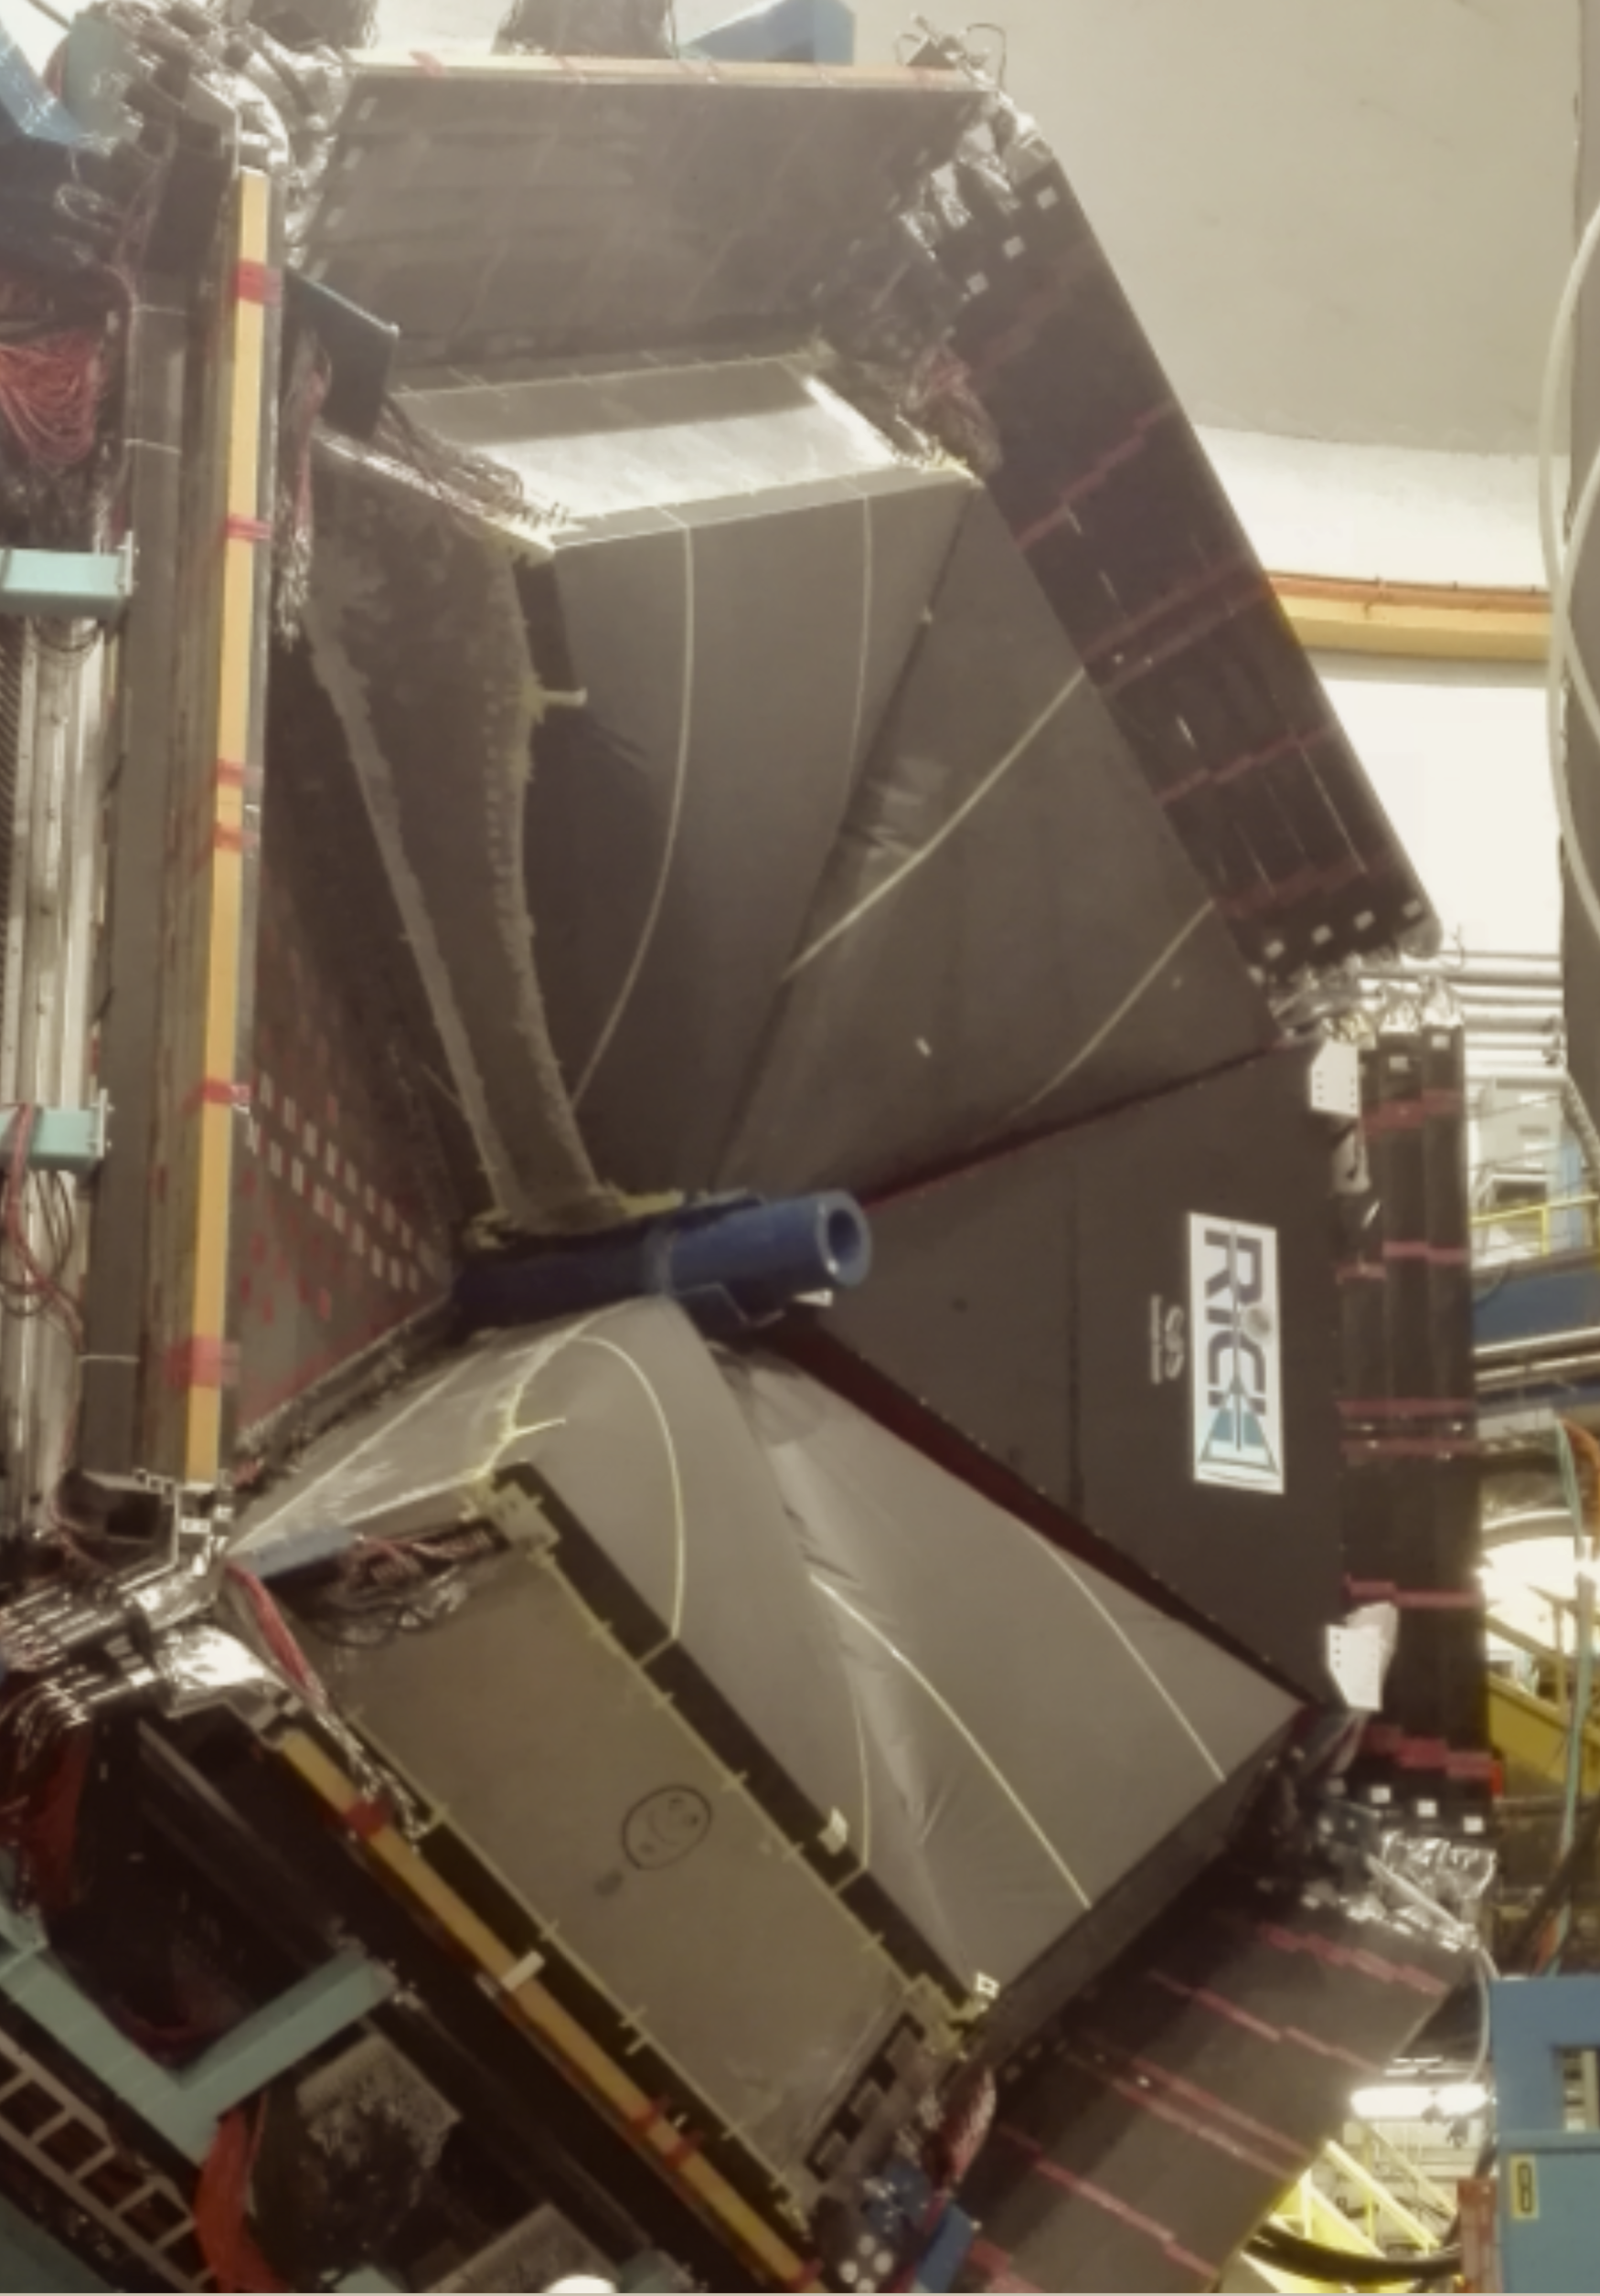
\includegraphics[width=1.0\columnwidth,keepaspectratio]{img/ltccInstalled.png}
    \caption{The LTCC sectors installed after refurbishment on the CLAS12 Forward Carriage. The RICH detector
    is installed in the sector~4 position and the sector~1 position awaits the installation of a second RICH detector.}
    \label{fig:ltccInstalled}
\end{figure}

\section{Acknowledgments}

We thank the Detector Support Group at Jefferson Lab for the work on the cone refurbishment, reflectivity tests,
PMT divider modifications and installation, and for designing the gas control system and associated software. We
thank Temple University for the p-terphenyl deposition. We thank Vladimir Popov for the implementation of the
divider base modification. We thank Youri Sharabian and Steve Christo for their consultations and contributions.
We thank the technical team of Hall~B for their work and dedication on all aspect of the project. Finally, we thank
all the Hall~B staff for their unyielding support. This work was supported in part by
DOE Contract DE-AC05-84ER40150.


\section{References}

\bibliography{bibfile}
\bibliographystyle{elsarticle-num}

\end{document}








